\documentclass[12pt]{article}
\usepackage{amsmath, amssymb, amsthm, graphicx, geometry, listings, xcolor, url, enumitem, fancyhdr, multirow}
\geometry{margin=1in}
\definecolor{darkgreen}{rgb}{0,0.5,0}
\pagestyle{fancy}

\lstset{
    frame=tb,
    language=Python,
    aboveskip=3mm,
    belowskip=3mm,
    showstringspaces=false,
    columns=flexible,
    basicstyle={\small\ttfamily},
    numbers=none,
    numberstyle=\tiny\color{green},
    keywordstyle=\color{blue},
    commentstyle=\color{darkgreen},
    stringstyle=\color{orange},
    breaklines=true,
    breakatwhitespace=true,
    tabsize=3
}

\lhead{SFSU, CSC 671-01}
\chead{Spring 2025}
\rhead{Deep Learning}

\title{Matrix Multiplication: PyTorch vs. Plain Python Performance Comparison}
\author{Bryan Lee\\922649673}
\date{February 12, 2025}

\begin{document}

\maketitle
\thispagestyle{fancy}

\section{Introduction}
One of the well-known facts about Python is its relatively slow speed when performing large computational tasks.
Compared to other popular programming languages like C++, Java, and even Node.js, Python tends to be slower in execution.
One key reason for this performance difference is that Python is an interpreted language, meaning that while it first compiles code into byte code,
it still executes instructions line by line at runtime rather than compiling everything into machine code beforehand.
Everything is also stored as objects, even in lists.
However, this limitation can be mitigated through specialized optimizations and external libraries.
For instance, libraries like PyTorch use a data structure called a tensor to represent matrices.
Tensors store data of a uniform type in contiguous memory, rather than as a collection of objects like Python lists.
PyTorch can also leverage GPU acceleration to further improve performance compared to standard Python.

\section{Preliminaries}
Matrix multiplication is a common linear algebra operation in numerical computing and machine learning.
It can be defined as a binary operation that produces a new matrix from two existing matrices.
The said matrix multiplication process can be described as follows: \\

\noindent Let $A \in \mathbb{R}^{m \times n}$, $B \in \mathbb{R}^{n \times p}$, and $C \in \mathbb{R}^{m \times p}$,

\begin{equation*}
    \begin{bmatrix}
        a_{11} & a_{12} & \cdots & a_{1n} \\
        a_{21} & a_{22} & \cdots & a_{2n} \\
        \vdots & \vdots & \ddots & \vdots \\
        a_{m1} & a_{m2} & \cdots & a_{mn}
    \end{bmatrix}
    \begin{bmatrix}
        b_{11} & b_{12} & \cdots & b_{1p} \\
        b_{21} & b_{22} & \cdots & b_{2p} \\
        \vdots & \vdots & \ddots & \vdots \\
        b_{n1} & b_{n2} & \cdots & b_{np}
    \end{bmatrix}
    =
    \begin{bmatrix}
        c_{11} & c_{12} & \cdots & c_{1p} \\
        c_{21} & c_{22} & \cdots & c_{2p} \\
        \vdots & \vdots & \ddots & \vdots \\
        c_{m1} & c_{m2} & \cdots & c_{mp}
    \end{bmatrix}
\end{equation*}

\noindent The product C consist of:

\begin{equation*}
    c_{ij} = a_{i1}b_{1j} + a_{i2}b_{2j} + \cdots + a_{in}b_{nj} = \sum_{k=1}^{n} a_{ik}b_{kj},
\end{equation*}

\noindent for \( i = 1, ..., m \) and j = \( 1, ..., p \). \\

\noindent\rule{\textwidth}{0.4pt}
\noindent\textbf{Matrix multiplication implementation in plain Python:}
\begin{lstlisting}
def multiplyMatrices(A: list[list[float]], B: list[list[float]]) -> list[list[float]]:
    """
        Multiplies two matrices A and B using plain python for-loops.
    """
    if len(A[0]) != len(B):
        raise ValueError("Matrix dimensions are not compatible: number of columns of matrix A must equal the number of rows of matrix B!");

    # Init result matrix with all 0s
    C = [[0 for _ in range(len(B[0]))] for _ in range(len(A))];

    # Perform matrix multiplication
    for i in range(len(A)):
        for j in range(len(B[0])):
            for k in range(len(B)):
                C[i][j] += A[i][k] * B[k][j];
    
    return C;
\end{lstlisting}

\noindent \\

As we can see, the algorithm runs in O(\( n^3 \)) time complexity, which is an expensive operation.
Additionally, the space complexity is also a concern, as each element in a plain Python list is stored as a separate object,
leading to increased memory occupation.
That begs the differ, how can we improve the computational speed of doing matrix multiplication?

As previously discussed, PyTorch has become a prominent tool in deep learning due to its flexibility and efficiency.
While NumPy arrays are similar to PyTorch's tensor, NumPy is more suited for general-purpose array computing.
It has limitations in deep learning applications, particularly because it lacks support for automatic differentiation and GPU acceleration.
On the other hand, PyTorch's tensor is specifically designed for deep learning applications,
so that will be the focus of our comparison.

\section{Approach}
To start, we will define a helper function that will generate two matrices, W and X, where
W is a \( 90 \times m \) matrix, and X is a \( m \times 110 \) matrix, where
\( m \in \{10, 20, ..., 100\} \).

\newpage

\noindent\rule{\textwidth}{0.4pt}
\noindent\textbf{Creating the randomized matrices:}
\begin{lstlisting}
import random

def generateMatrices(m: int) -> tuple[list[list[float]], list[list[float]]]:
    W = [[random.random() for _ in range(m)] for _ in range(90)];
    X = [[random.random() for _ in range(110)] for _ in range(m)];

    return W, X;
\end{lstlisting}

\noindent \\

\noindent The main experiment script iterates through each pair of generated \( W \) and \( X \) matrices,
corresponding to different \( m \) values, and constructs their tensor counterparts.
It then utilizes IPython's timeit magic command to conduct seven runs of matrix multiplication for both the plain Python and vectorized implementations.
The average runtime from these runs provides a more precise estimate of each implementation's runtime performance.

\noindent\rule{\textwidth}{0.4pt}
\noindent\textbf{Running the 10 timing experiments:}
\begin{lstlisting}
import torch

def convertToTensor(W, X):
    W_t = torch.tensor(W);
    X_t = torch.tensor(X);

    return W_t, X_t;

m_vals = [m for m in range(10, 110, 10)];
matrices = [generateMatrices(m) for m in m_vals];

pyTimeResults = [];
tensorTimeResults = [];
for W, X in matrices:
    # Create the tensor matrices
    W_t, X_t = convertToTensor(W, X);

    # Time the plain Python matrix multiplication
    pythonTime = %timeit -o multiplyMatrices(W, X);
    pyTimeResults.append(pythonTime.average);

    # Time the torch matrix multiplication
    tensorTime = %timeit -o W_t.matmul(X_t);
    tensorTimeResults.append(tensorTime.average);
\end{lstlisting}

\noindent \\

\noindent The timeit function produces an output for each iteration, shown below.
The table reveals that, in the plain Python implementation, the magic function is executed only 10 times, while PyTorch runs it 10,000 times.
Additionally, the time per loop is considerably lower for the PyTorch implementation, highlighting its superior speed for matrix multiplication.

\begin{table}[ht]
    \centering
    \begin{tabular}{|c|c|c|}
        \hline
        \multirow{2}{*}{\textbf{Iteration with m value}} & \multicolumn{2}{c|}{\textbf{Per loop (mean ± std. dev.)}} \\
        \cline{2-3}
            & 10 loops each (Plain Python) & 10,000 loops each (PyTorch) \\
        \hline
        10  & 21.9 ms $\pm$ 1.63 ms  & 24.7 $\mu$s $\pm$ 7.46 $\mu$s  \\
        \hline
        20  & 40.7 ms $\pm$ 4.84 ms  & 24.4 $\mu$s $\pm$ 1.44 $\mu$s  \\
        \hline
        30  & 55.6 ms $\pm$ 813 $\mu$s  & 24.9 $\mu$s $\pm$ 1.05 $\mu$s  \\
        \hline
        40  & 72.6 ms $\pm$ 635 $\mu$s  & 27.1 $\mu$s $\pm$ 2.72 $\mu$s  \\
        \hline
        50  & 92.0 ms $\pm$ 4.04 ms  & 29.1 $\mu$s $\pm$ 1.48 $\mu$s  \\
        \hline
        60  & 109 ms $\pm$ 4.53 ms  & 30.8 $\mu$s $\pm$ 1.64 $\mu$s  \\
        \hline
        70  & 126 ms $\pm$ 1.54 ms  & 33.3 $\mu$s $\pm$ 1.86 $\mu$s  \\
        \hline
        80  & 144 ms $\pm$ 3.98 ms  & 35.3 $\mu$s $\pm$ 1.68 $\mu$s  \\
        \hline
        90  & 162 ms $\pm$ 4.22 ms  & 38.9 $\mu$s $\pm$ 3.51 $\mu$s  \\
        \hline
    \end{tabular}
    \caption{Performance metrics for different m values.}
\end{table}

\noindent There is an edge case for the last iteration with \( m = 100 \),
where the plain Python implementation executes only 1 loop.
This is likely due to performance and bottleneck considerations
when handling such a large computation.

\begin{table}[ht]
    \centering
    \begin{tabular}{|c|c|c|}
        \hline
        \multirow{2}{*}{\textbf{Iteration with m value}} & \multicolumn{2}{c|}{\textbf{Per loop (mean ± std. dev.)}} \\
        \cline{2-3}
        & 1 loop (Plain Python) & 10,000 loops (PyTorch) \\
        \hline
        100 & 179 ms $\pm$ 2.87 ms & 41.8 $\mu$s $\pm$ 8.09 $\mu$s \\
        \hline
    \end{tabular}
    \caption{Performance metrics for m value of 100.}
\end{table}

\noindent We can also see the significant difference between plain Python and PyTorch when we
print out the average of the timeit function below.

\noindent\rule{\textwidth}{0.4pt}
\noindent\textbf{Displaying the average time results for the matrix multiplication experiment:}
\begin{lstlisting}
print("Average Time results for timeit tests on regular python matrices:");
print(pyTimeResults);

Average Time results for timeit tests on regular python matrices:
[0.02194325428572483, 0.04067932000034489, 0.05562064714301544, 0.07257928000014675, 0.0919591871429085, 0.10945918000028801, 0.12607538285686, 0.14421578714245697, 0.16206269857128583, 0.17928888571415363]

print("Average Time results for timeit tests on tensor matrices:");
print(tensorTimeResults);

Average Time results for timeit tests on tensor matrices:
[2.469240571476153e-05, 2.4358931428495062e-05, 2.4857308571725818e-05, 2.7050777142825868e-05, 2.912901999994314e-05, 3.0784302856981025e-05, 3.328427285700205e-05, 3.5271571428373656e-05, 3.8860460000536737e-05, 4.182551857167189e-05]
\end{lstlisting}

\section{Visualizing the Results}
Using the retrieved data, we will plot the speed improvement ratio between the plain Python and PyTorch implementations, calculated using the following formula:

\begin{equation*}
    \text{speed improvement ratio} = \sum_{i = 0}^{i < n} \frac{\text{pyTimeResults[i]}}{\text{tensorTimeResults[i]}}
\end{equation*}

\noindent Additionally, I will also compute the line of best fit for the data points using the least squares method.
It will be computed as follows:

\begin{equation*}
    A = 
    \begin{bmatrix}
        1 & 10 \\
        1 & 20 \\
        \vdots & \vdots \\
        1 & 100
    \end{bmatrix},\quad
    b =
    \begin{bmatrix}
        \text{speed\_improvement\_ratio[0]} \\
        \text{speed\_improvement\_ratio[1]} \\
        \vdots \\
        \text{speed\_improvement\_ratio[9]} \\
    \end{bmatrix}
\end{equation*}

\noindent Where A is a vertical matrix with the first column consisting of all ones, and the second column consisting of the m values.
On the other hand, b is a vertical vector of the speed improvement ratio values. Now for the computation:

\begin{equation*}
    x^* = (A^T A)^{-1} A^T b
\end{equation*}

\noindent Giving us the line of best fit line:

\begin{equation*}
    bestFitLine(m) = \alpha + \beta * m
\end{equation*}

\newpage

\noindent\rule{\textwidth}{0.4pt}
\noindent\textbf{Plotting the speed improvement graph:}
\begin{lstlisting}
import matplotlib.pyplot as plt
import numpy as np

speedImprovementRatio = [py / tensor for py, tensor in zip(pyTimeResults, tensorTimeResults)];

# Compute the line of best fit using least squares solution
A = np.column_stack((np.ones(len(m_vals)), m_vals)); # Col of 1s and m_vals
b = np.array(speedImprovementRatio); # Vertical vector of ratios

x_star = np.linalg.inv(A.T @ A) @ (A.T @ b); # x* = (A' * A)^-1 * A' * b

alpha = x_star[0];
beta = x_star[1];

bestFitLine = [alpha + beta * m for m in m_vals]; # Formulate the best fit line

plt.plot(m_vals, speedImprovementRatio, color='b', label="Speed Improvement");
plt.plot(m_vals, bestFitLine, color='r', label="Best Fit Line");

plt.xlabel("Matrix Size (m)");
plt.ylabel("Speed Improvement Ratio (Plain / Vectorized)");
plt.title("Speed Improvement of PyTorch Vectorized Multiplication Over Plain Python");
plt.legend();
plt.show();
\end{lstlisting}

\newpage

\begin{figure}[ht]
    \centering
    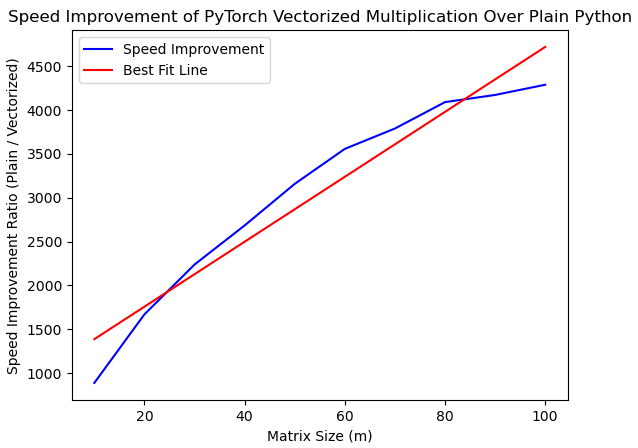
\includegraphics[width=1\linewidth]{PythonVSPyTorch.PNG}
    \caption{Speed improvement ratio of PyTorch over Plain Python.}
\end{figure}

\noindent Additionally, for a more adherent difference, we will be plotting the time difference between the two implementations.

\noindent\rule{\textwidth}{0.4pt}
\noindent\textbf{Plotting the time difference:}
\begin{lstlisting}
plt.plot(m_vals, [p for p in pyTimeResults], color='b', label="Plain Python");
plt.plot(m_vals, [t for t in tensorTimeResults], color='r', label="PyTorch Tensor");

# plt.xticks(m_vals);
plt.xlabel("Matrix Size (m)");
plt.ylabel("Time (s)");
plt.yscale("log");
plt.title("Matrix Muliplication Time Comparison");
plt.legend();
plt.show();
\end{lstlisting}

\newpage

\begin{figure}[ht]
    \centering
    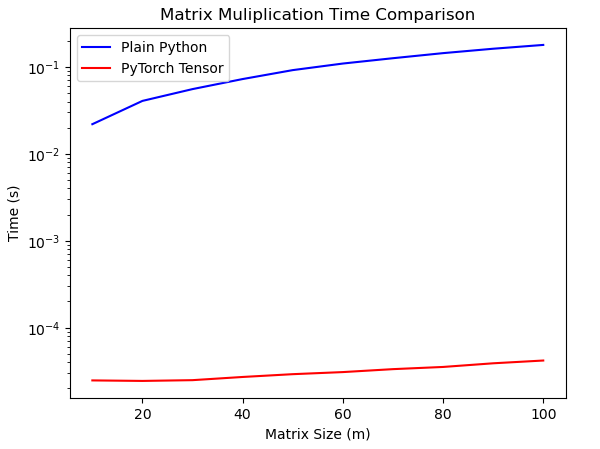
\includegraphics[width=1\linewidth]{TimeDiffPythonVsPyTorch.PNG}
    \caption{Time difference between PyTorch over Plain Python.}
\end{figure}

\noindent We can see that tensors appear to be operating with a run time speed closer to a logarithmic scale (flatter line), meaning that it has better performance for large matrices.

\section{Conclusion}
In conclusion, the experiments clearly demonstrate that using PyTorch tensors for matrix multiplication provides a substantial performance boost compared to the plain Python implementation.
While some variation exists due to standard deviations, the PyTorch implementation consistently outperforms its plain Python counterpart.
By enforcing a homogeneous data type for tensors, computation time is significantly reduced.
Additionally, this approach minimizes the need to reference new objects for each matrix element and compacts data storage by nearly sixfold.
These optimizations are crucial for deep learning applications, where efficient matrix operations are essential for handling large-scale computations.

\newpage

\begin{thebibliography}{4}
    \bibitem{Internal working of Python}
    GeeksforGeeks. (2023). \textit{Internal working of Python}. \url{https://www.geeksforgeeks.org/internal-working-of-python/}.
    
    \bibitem{PyTorch Tensor vs Numpy Array}
    GeeksforGeeks. (2024). \textit{PyTorch Tensor vs Numpy Array}. \url{https://www.geeksforgeeks.org/pytorch-tensor-vs-numpy-array/}.

    \bibitem{Why tensors perform insanely faster than lists?}
    Radovich, V. (2024). \textit{Why tensors perform insanely faster than lists? -- An introduction to storage}. https://medium.com/@valentinradovich/why-tensors-perform-insanely-faster-than-lists-an-introduction-to-storage-bf36723bbaf2.


    \bibitem{Wikipedia Matrix Multiplication}
    Wikimedia Foundation. (2024). \textit{Matrix multiplication}. Wikipedia. \url{https://en.wikipedia.org/wiki/Matrix_multiplication}.
\end{thebibliography}


\end{document}
